\documentclass[twoside]{report}
\usepackage{anyfontsize}
\usepackage{fancyhdr}
\usepackage[papersize={9in, 11in}, margin=.6in]{geometry}
\usepackage[dvipsnames, svgnames]{xcolor}
\usepackage{multicol}
\usepackage{multicol}
\usepackage{pagecolor}
\usepackage{titlesec}
\usepackage{tikz}
\usepackage{background}

\newcommand{\centered}[1]{\begin{tabular}{l} #1 \end{tabular}}

\newcommand{\bioEntry}[2]{

\begin{tabular}{c c}
	\raisebox{-.5\height}{
	\roundpic{4cm}{4cm}{#1}} & 
	\centered{\fontsize{16}{16}\selectfont #2}\\
\end{tabular}

}

\renewcommand{\headrulewidth}{0pt}

\pagenumbering{arabic}
\fancyhf{}
\titleformat{\section}{\fontsize{22}{22}\selectfont\bfseries}{}{0em}{}

\makeatletter
\newcommand{\addchapter}[1]{%
  \begingroup
  \let\@makechapterhead\@gobble % make \@makechapterhead do nothing
  \addcontentsline{toc}{chapter}{#1}
  \endgroup
}
\makeatother


\newcommand{\secCol}{Black}
\newcommand{\txtCol}{Black}

\begin{document}\fontsize{12}{12}\selectfont
\pagenumbering{gobble}
\pagecolor{brown}

\backgroundsetup{
scale=1,
angle=0,
opacity=2,  %% adjust
contents={
\includegraphics[width=\paperwidth,height=\paperheight]{images/cover.jpg}}
}
\begin{titlepage}
{\fontsize{1}{1}\selectfont blank text}
\end{titlepage}
\vfill
\newpage

\backgroundsetup{
scale=1,
angle=0,
opacity=0,
contents={}
%\includegraphics[width=\textwidth]{Cover-Image.png}
}

\pagenumbering{arabic}
\pagestyle{fancy}
\fancyhead[LO, RE]{\fontsize{20}{20}\selectfont\thepage}
%\fancyhead[EL]{\fontsize{20}{20}\selectfont\thepage}
\pagecolor{white}

\tableofcontents

{\begin{center}\fontsize{48}{48}\selectfont
\textcolor{white}{\textbf{Meet the Authors}}
\end{center}}
\vspace{.75in}
\bioEntry{images/headshot.jpg}{0}{0}{1.25cm}{0}{0}{1in}{Joshua Bays [BIO]}\vspace{1cm}\noindent
\bioEntry{images/cat.jpg}{0}{0}{1.25cm}{0}{0}{1in}{Kitty Cat [BIO]}\vspace{1cm}\noindent
%\bioEntry{cat.png}{Damien Brack [BIO]}\vspace{1cm}\noindent
%\bioEntry{black.jpg}{Nick Brownfield [BIO]}\vspace{1cm}\noindent
%\bioEntry{black.jpg}{Josh Caruso [BIO]}\vspace{1cm}\noindent
%\bioEntry{black.jpg}{Jordan Lochow [BIO]}\vspace{1cm}\noindent
%\bioEntry{black.jpg}{Kanako Walker [BIO]}\vspace{1cm}\noindent
%\bioEntry{black.jpg}{Michael Williams [BIO]}\vspace{1cm}\noindent
%\bioEntry{black.jpg}{Alex Wood [BIO]}\vspace{1cm}\noindent
%\bioEntry{black.jpg}{Asmma Zaitar [BIO]}\vspace{1cm}\noindent


\renewcommand{\secCol}{Brown}
\renewcommand{\txtCol}{Black}
\pagecolor{Apricot}

\addchapter{Peanut Butter and Jelly Sandwiches}
{\begin{center}\fontsize{48}{48}\selectfont
\textcolor{Bittersweet}{\textbf{Peanut Butter and Jelly Sandwiches}}
\end{center}}

\begin{center}
\vspace{.25in}
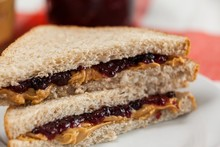
\includegraphics[height=1.5in]{images/pbj.jpg}
\end{center}

\textcolor{\secCol}{\section*{Ingredients}}\fontsize{12}{12}\selectfont\textcolor{\txtCol}{\textbf{
\begin{multicols}{2}
\begin{enumerate}
\item Peanut butter
\item Jelly
\item 2 slices of bread
\item INGREDIENT
\item INGREDIENT
\item INGREDIENT
\item INGREDIENT
\item INGREDIENT
\item INGREDIENT
\\
\end{enumerate}
\end{multicols}
}}

\textcolor{\secCol}{\section*{Instructions}}\fontsize{12}{12}\selectfont\textcolor{\txtCol}{\textbf{
\begin{multicols}{2}
\begin{enumerate}
\item Put the peanut butter on a slice of bread
\item Put the jelly on the piece of bread
\item Put the 2 bread slices together
\item INSTRUCTIONS
\item INSTRUCTIONS
\item INSTRUCTIONS
\item INSTRUCTIONS
\item INSTRUCTIONS
\item INSTRUCTIONS
\\
\end{enumerate}
\end{multicols}
}}

\textcolor{\secCol}{\section*{Cultural Context}}\fontsize{14}{14}\selectfont
\noindent\textcolor{\txtCol}{
Peanut Butter and Jelly Sandwiches are an essential part of any traditional suburban American household.
Strawberry jelly is the better way, but grape jelly is acceptable.
\\
}


\renewcommand{\secCol}{White}
\renewcommand{\txtCol}{Sepia}
\pagecolor{CarnationPink}

\addchapter{Ham and Cheese Sandwiches}
{\begin{center}\fontsize{48}{48}\selectfont
\textcolor{RoyalPurple}{\textbf{Ham and Cheese Sandwiches}}
\end{center}}

\begin{center}
\vspace{.25in}
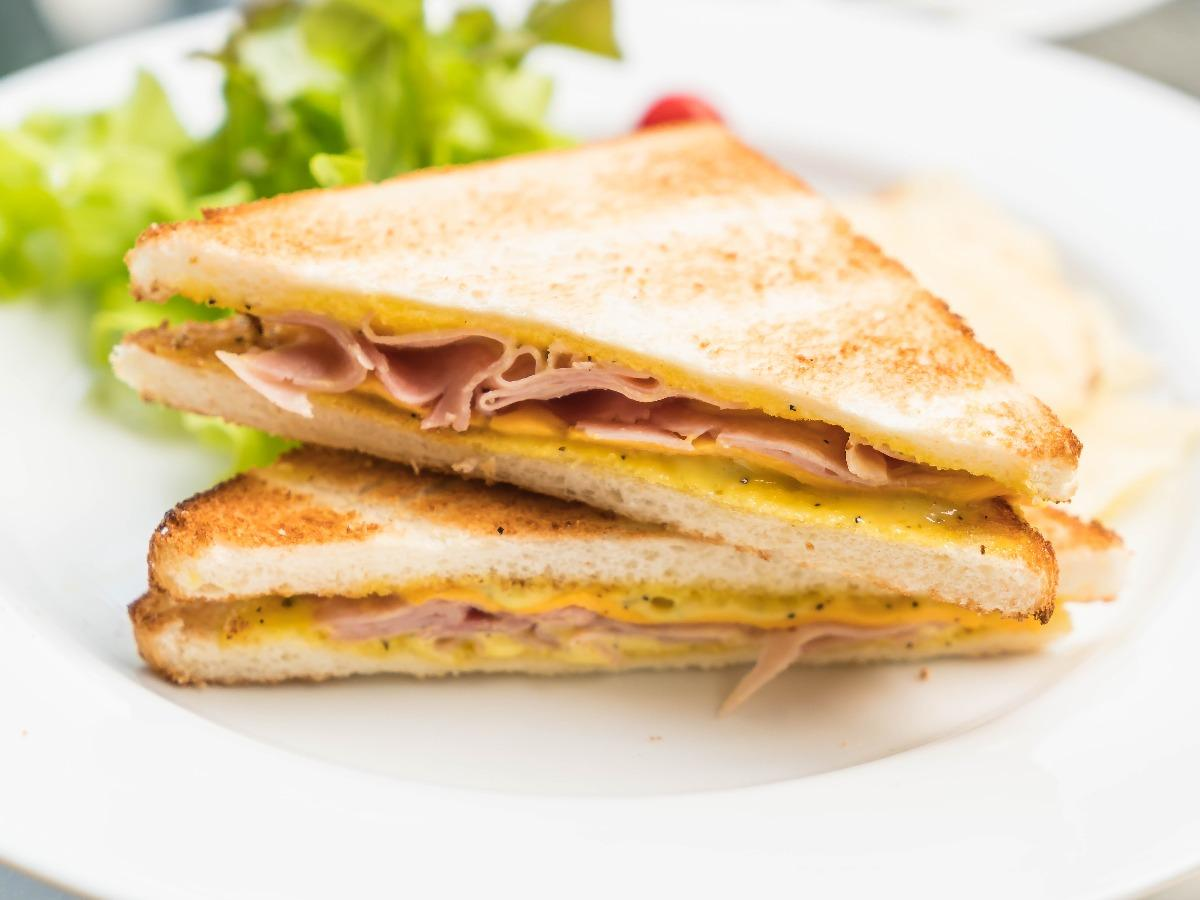
\includegraphics[height=1.5in]{images/hamcheese.jpg}
\end{center}

\textcolor{\secCol}{\section*{Ingredients}}\fontsize{12}{12}\selectfont\textcolor{\txtCol}{\textbf{
\begin{multicols}{2}
\begin{enumerate}
\item Ham
\item Cheese
\item 2 slices of bread
\item INGREDIENT
\item INGREDIENT
\item INGREDIENT
\item INGREDIENT
\item INGREDIENT
\item INGREDIENT
\\
\end{enumerate}
\end{multicols}
}}

\textcolor{\secCol}{\section*{Instructions}}\fontsize{12}{12}\selectfont\textcolor{\txtCol}{\textbf{
\begin{multicols}{2}
\begin{enumerate}
\item Put the peanut butter on a slice of bread
\item Put the jelly on the piece of bread
\item Put the 2 bread slices together
\item INSTRUCTIONS
\item INSTRUCTIONS
\item INSTRUCTIONS
\item INSTRUCTIONS
\item INSTRUCTIONS
\item INSTRUCTIONS
\\
\end{enumerate}
\end{multicols}
}}

\textcolor{\secCol}{\section*{Cultural Context}}\fontsize{14}{14}\selectfont
\noindent\textcolor{\txtCol}{
Ham and cheese Sandwiches are an essential part of any traditional suburban American household.
You can also use turkey.
\\
}



\end{document}
